% Template for Cogsci submission with R Markdown

% Stuff changed from original Markdown PLOS Template
\documentclass[10pt, letterpaper]{article}

\usepackage{cogsci}


\title{Noun bias, revisited: Investigating syntactic category bias in
early bilingual vocabularies}


\author{{\large \bf Alvin Wei Ming Tan (tanawm@stanford.edu)} \\ Department of Psychology \\ Stanford University \AND {\large \bf Michael C. Frank} \\ Department of Psychology \\ Stanford University}


\begin{document}

\maketitle

\begin{abstract}
Why are nouns often over-represented in children's early words? Prior
research has suggested a range of possible explanations for the observed
bias in the syntactic category composition of early vocabularies,
including cognitive, linguistic, and contextual factors. In this study,
we attempted to disambiguate the contributions of such factors by
studying the vocabularies of children acquiring two languages. Across
three analyses (\(N\) = 1997), we investigated the role of different
language combinations, different levels of language exposure, and
different environmental contexts, finding some support for
cross-linguistic modulation of syntactic category bias, as well as
variation across countries. These results suggest that multiple
interacting factors contribute to syntactic category biases in young
children's vocabularies, and highlight the importance of understanding
the broader background of the child when studying language acquisition.

\textbf{Keywords:}
bilingualism; vocabulary; noun bias
\end{abstract}

\section{Introduction}\label{introduction}

Children's vocabularies are an important lens into the factors that
shape language learning, including language input, learning
environments, and cognitive biases. One way to analyse such early
vocabularies is to examine their composition in terms of syntactic
categories. Prior research has suggested that early vocabularies are
dominated by words for objects, rather than words for relations; this is
known as the noun bias, and has been reported for a wide range of
languages (e.g., Bornstein et al., 2004; Gentner, 1982; see Waxman et
al., 2013 for a review). Nonetheless, there has also been evidence
suggesting that some languages exhibit no such noun bias, including
Mandarin (Tardif, 1996), Korean (Choi \& Gopnik, 1995), and Tseltal
(Casillas et al., 2024) among others. Furthermore, different studies
have found conflicting results even for the same language (e.g., compare
Bornstein et al. (2004) and Choi \& Gopnik (1995) for Korean).
Considering the variation in results, there remain important theoretical
questions about explanations for the occurrence of the noun bias in some
(but probably not all) early vocabularies.

Hypothesised accounts for the observed noun bias fall into three broad
domains. The first domain focuses on the \emph{cognitive} process of
word learning, proposing that nouns are easier to encode than
predicates. Gentner's (1982) natural partitions/relational relativity
hypothesis suggests that objects are perceptually individuable (and thus
easier to map to labels), whereas relations are individuated only via
linguistic selection (and thus take more time to learn). The second
domain relates to \emph{linguistic} features affecting whether nouns or
predicates are easier to learn. Such explanations include the suggestion
that, relative to predicates, nouns are more frequent in child-directed
speech (e.g., Goldfield, 1993; Kim et al., 2000), nouns are less
morphologically complex (e.g., Tardif et al., 1997), or nouns are more
salient (e.g., Caselli et al., 1995). Crucially, this domain seeks to
account for the observed variation in the noun bias across languages,
since the posited features vary across languages. The third domain is
\emph{contextual}, suggesting that sociocultural features influence how
nouns and predicates are communicated about or processed. For example,
different cultures may emphasise labels to differing extents (e.g., Choi
\& Gopnik, 1995; Tardif et al., 1999), or may have differential patterns
of attention towards objects or relations (e.g., Lavin et al., 2006;
Waxman et al., 2016). Notably, these three domains of explanation are
not mutually exclusive, and multiple sets of features may jointly
influence the learning of words across syntactic categories. However, it
is typically difficult to distinguish between linguistic and contextual
factors, since they tend to covary.

One way to disentangle linguistic and contextual factors is by studying
bilingual children, who serve as a ``natural experiment'', since they
reside within a single context while acquiring two languages; in other
words, contextual factors are constant while linguistic factors vary
across their two languages. Previous research have shown that bilingual
children exhibit differently sized noun biases in their two languages;
this effect has been attested in English--Mandarin bilinguals (Chan \&
Nicoladis, 2010; Levey \& Cruz, 2003; Setoh et al., 2021; Xin \& Lucas,
2010; Xuan \& Dollaghan, 2013), Filipino--English bilinguals (Lucas \&
Bernardo, 2008) and Turkish--Dutch bilinguals (Özcan et al., 2016). The
language-specific bias may depend on the specific language combination,
however, as no such effect was found for a Portuguese--English bilingual
child (Nicoladis, 2001) or a German--Italian bilingual child (Klammler
\& Schneider, 2011)---although it should be noted that these are case
studies and may not have sufficient generalisability or power.
Additionally, Chai et al. (2021) has shown that bilinguals learning
different language combinations (English--Mandarin vs English--Malay)
can show differently sized noun biases in the common language (in this
case, English), suggesting that there is some cross-linguistic
influence, perhaps due to the preferential learning of translation
equivalents (e.g., ``dog'' in English and ``perro'' in Spanish) (e.g.,
Tan et al., 2024; Tsui et al., 2022). Different levels of language
exposure have also been shown to affect noun bias sizes in
Basque--Spanish bilingual children (Barnes \& Garcia, 2013). Together,
these results suggest that linguistic (and cross-linguistic) factors
must play a role in explaining the noun bias, since variation across
languages persists even when cognition and context are controlled for.

Surveying prior observational research on the noun bias, however,
reveals another dimension of variation, namely analytic heterogeneity,
which may explain some of the variance in the results obtained. Some
studies have used direct counts of the number of nouns or predicates
known by a child (e.g., Levey \& Cruz, 2003; Özcan et al., 2016, ;
Tardif et al., 1997). Other studies have measured nouns or predicates
known as a proportion of the child's vocabulary (e.g., Bornstein et al.,
2004; Chan \& Nicoladis, 2010; Choi \& Gopnik, 1995, ; Gentner, 1982). A
third option is the use of a ratio---for example, the ratio of nouns to
the sum of nouns and predicates (e.g., Chai et al., 2021; Setoh et al.,
2021; Tardif et al., 1999). However, each of these three approaches is
potentially affected by an availability problem: if there are more nouns
than verbs that are \emph{available} for a child to learn, it would not
be surprising for them to have more nouns in their vocabulary (whether
by count, proportion, or ratio) even if they were acquiring words
entirely by chance. In other words, when evaluating whether children
have tendencies to prefer learning nouns over predicates, our key metric
of interest should be whether children know more nouns \emph{than would
be expected}---i.e., whether there is an \emph{over-representation} of
nouns in the child's vocabulary.

To study the over- or under-representation of syntactic categories in
early bilingual vocabularies, we adopted the approach taken by Bates et
al. (1994) and Frank et al. (2021). This approach used data from
parent-report vocabulary checklists, and children's known words are
expressed as proportions of the total number of words in that category
on the checklist (i.e., potential opportunities for word learning). This
is then plotted against children's total vocabularies, again expressed
as proportions of the total size of the checklist. If children were to
acquire words independently of their syntactic category, then we would
expect their category proportions to match their total vocabulary
proportions. Conversely, if children had a noun bias, then their noun
proportions should exceed their total vocabulary proportions, suggesting
an over-representation of nouns in their vocabularies. Such an analytic
approach would thus control for the word learning opportunities that
children experience overall, allowing the specific investigation of
whether there are learning biases beyond mere variation in the
availability of learnable words.

The present study thus employs this over-/under-representation approach
to studying syntactic category biases in bilingual children, aiming to
disentangle the roles of linguistic and contextual factors in shaping
early vocabulary compositions. We consider the following (mutually
exclusive) alternative hypotheses regarding linguistic factors:

\begin{quote}
H1a: The category bias is entirely cognitive in origin. Hence,
individual bilingual children have same-sized category biases across
their two languages.
\end{quote}

\begin{quote}
H1b: The category bias is affected by linguistic factors. Hence,
bilingual children have different-sized category biases across their two
languages. However, there is no cross-linguistic influence, so bilingual
children have category biases comparable to monolinguals in each
language.
\end{quote}

\begin{quote}
H1c: The category bias is affected by linguistic factors, and
additionally can be modulated by cross-linguistic effects. Hence, for
each language learnt by a bilingual child, there is a shift in category
biases \emph{away from} monolinguals of that language, \emph{towards}
monolinguals of the other language.
\end{quote}

We also consider the following (mutually exclusive) alternative
hypotheses regarding contextual factors:

\begin{quote}
H2a: The category bias is not affected by contextual factors, and is
only affected by universal cognitive and/or linguistic factors. Hence,
bilingual children learning the same combination of languages but in
different environmental contexts should have same-sized category biases.
\end{quote}

\begin{quote}
H2b: The category bias is affected by contextual factors. Hence,
bilingual children learning the same combination of languages but in
different environmental contexts may exhibit different-sized category
biases.
\end{quote}

In the present study, we test these two sets of hypotheses through a set
of three analyses on data from early children's vocabularies to
understand the possible origin of the noun bias in young children's word
learning.

\section{Methods}\label{methods}

In this section, we describe the broad methodological approach for all
three analyses, leaving analysis-specific details to the subsequent
sections. All code is available at {[}REDACTED{]}.

\subsection{Vocabulary data}\label{vocabulary-data}

\begin{CodeChunk}
\begin{figure}[t]

{\centering 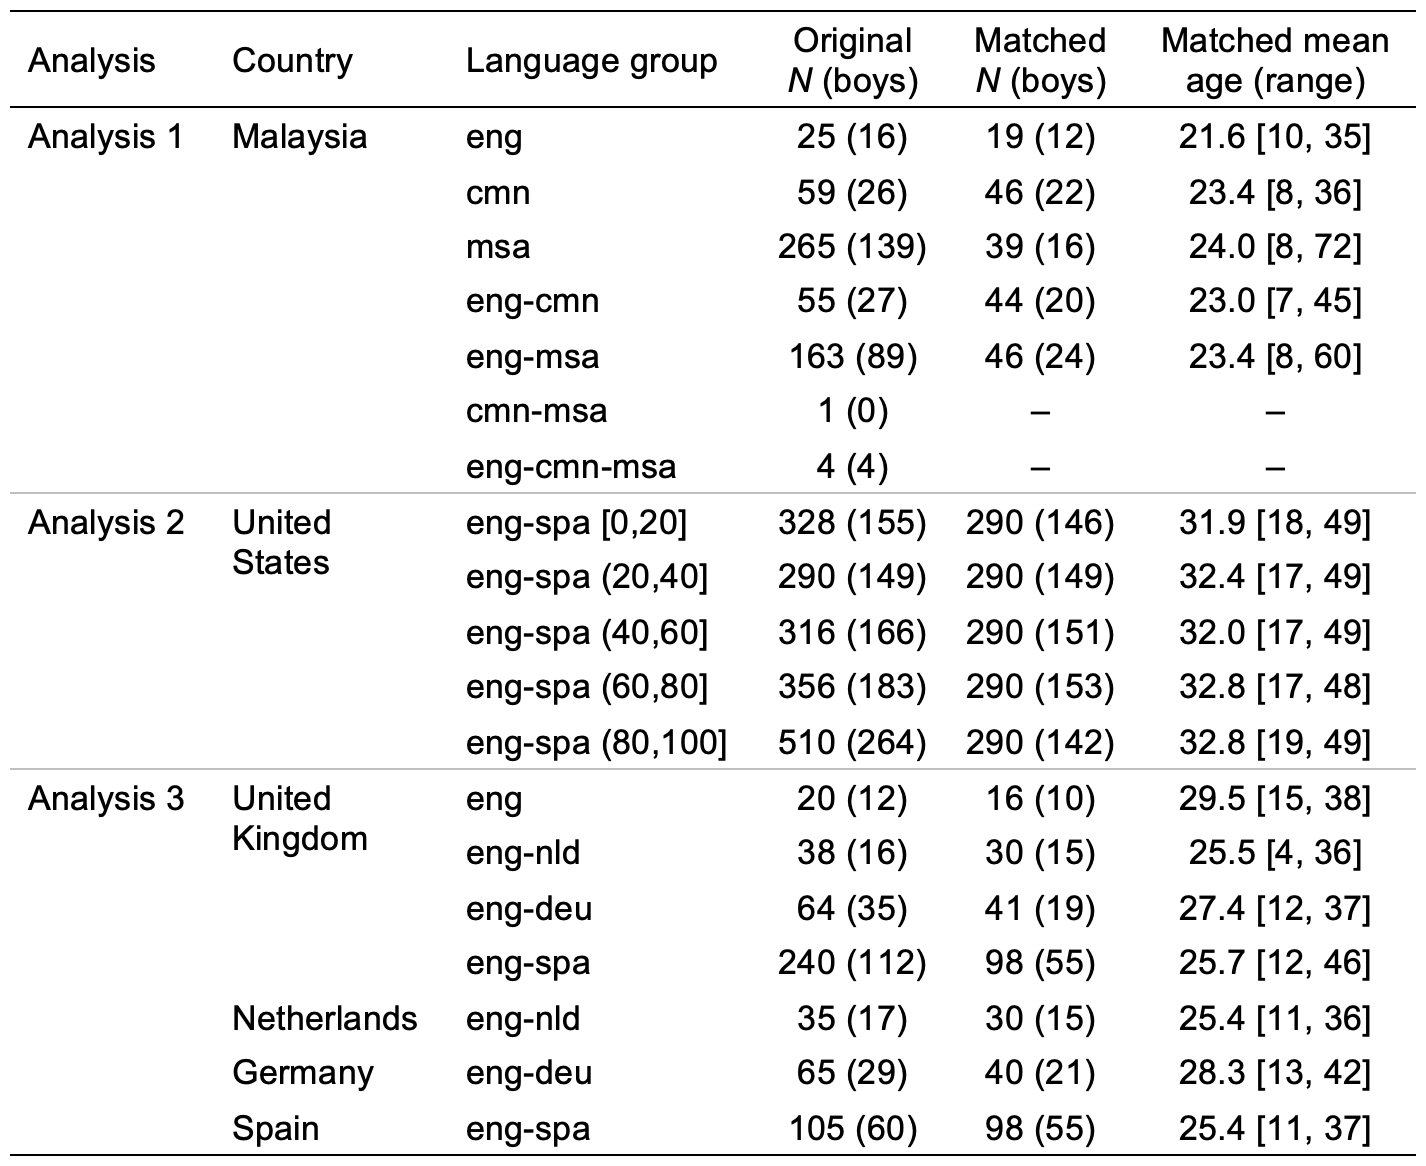
\includegraphics[width=240pt]{figs/demogs} 

}

\caption[Demographics of participants in all three analyses by country and language group]{Demographics of participants in all three analyses by country and language group. For Analysis 2, ranges indicate children's exposure proportions to English.}\label{fig:demogs}
\end{figure}
\end{CodeChunk}

We used data collected using Communicative Development Inventories
(CDIs), which are parent-report vocabulary checklists (Marchman et al.,
2023). CDIs have been used by researchers in many contexts due to their
ease of administration, their reliability and validity as a measure of
language ability, and their availability in many language- and
context-appropriate adaptations (Fenson et al., 2007; Mayor \& Plunkett,
2011). We obtained CDI data from Wordbank (Frank et al., 2017), an open
repository of CDI data that includes a few bilingual datasets. These
datasets contained vocabulary data for each child, as well as
demographic information including the child's age and sex. Each dataset
also included language exposure values, standardised as percentages of
exposure to each language. An overview of participant demographics for
all analyses is shown in Figure \ref{fig:demogs}. We focused on
production data for all analyses.

\subsection{Matching}\label{matching}

Several covariates are known to affect early vocabularies, including the
child's age and sex (Frank et al., 2021, ch.~6). To control for these
effects, we conducted matching across different groups (e.g.,
monolinguals vs bilinguals, or bilinguals of different backgrounds),
with the smallest group of interest as the focal group (i.e., common
referent matching, Rassen et al., 2011). We matched for age and sex as
covariates, as well as language exposure when comparing between
bilinguals of different language combinations or countries. We used
cardinality matching as the matching method, as it provides better
sample retention for small sample sizes (Fortin et al., 2021). We
verified the balance of the matched groups by evaluating the
standardised mean differences for covariates after matching, using 0.1
as the threshold for balance.

\subsection{Bias estimation}\label{bias-estimation}

We divided CDI items into four syntactic categories: nouns, predicates
(verbs and adjectives), function words (closed-class words), and other
(e.g., onomatopoeia and proper nouns); items in the other category were
excluded from further analyses. We then calculated the proportion of
items known for each syntactic category (e.g., the number of nouns known
divided by the total number of nouns on the CDI), as well as total
vocabulary as a proportion of all CDI items.

We can thus calculate a group-level bias by estimating a generalised
linear model predicting category proportion as a function of vocabulary
proportion, and measuring the area between this curve and the diagonal.
If the curve lay above the diagonal, this area would be positive,
indicating a positive bias, while if the curve lay below the diagonal,
this area would be negative, indicating a negative bias. Following
previous work (Frank et al., 2021, ch.~11), we used a third-order
polynomial model constrained to pass through (0, 0) and (1, 1). We also
estimated confidence intervals by resampling 10,000 times with
replacement for each group.

\subsection{Permutation testing}\label{permutation-testing}

To test if groups differed in their syntactic category biases, we
conducted permutation testing by shuffling group labels and
re-estimating the biases. For each analysis, we shuffled group labels
10,000 times and re-calculated the between-group differences in bias,
allowing for an estimation of the \(p\)-value of the true observed
between-group difference. We used a threshold of \(\alpha = .05\) for
significance. All \(p\)-values were adjusted for multiple comparisons
using Benjamini--Hochberg correction (Benjamini \& Hochberg, 1995).

\section{Analysis 1: Varying language
combinations}\label{analysis-1-varying-language-combinations}

Our first analysis attempted to understand if children with different
language combinations would exhibit different category biases. In
particular, we examined if bilinguals differed from monolinguals, and if
different types of bilinguals (Mandarin--English and Malay--English)
differed from each other, replicating Chai et al. (2021). This set of
language combinations is particularly interesting because Mandarin has
been suggested to have a positive verb bias and no noun bias, whereas
English has a positive noun bias and a negative verb bias (e.g., Frank
et al., 2021, ch.~11), and Malay was hypothesised to be more similar to
English than Mandarin (Chai et al., 2021). Hence, if syntactic category
bias can be cross-linguistically modulated, it should be apparent in
Mandarin--English bilinguals, whereas we do not expect the same
modulation for Malay--English bilinguals.

\subsection{Dataset}\label{dataset}

The dataset for this analysis was contributed by Chai et al. (2021). It
includes 572 children (301 boys) from Malaysia aged 6--72 months. We
thresholded the language exposure values at 10\% (i.e., participants
with \textless10\% exposure to a language were considered to not be
exposed to that language), and divided the participants into groups
based on the languages they were exposed to (some subset of Mandarin,
Malay, and English). Some groups were too small and were omitted
(Mandarin--Malay bilinguals and Mandarin--Malay--English trilinguals);
we used matching over the remaining groups, with Mandarin--English
bilinguals as the focal group.\footnote{Note that the monolingual
  English group was in fact smaller than the Mandarin--English bilingual
  group, but matching to that group resulted in a much smaller final
  sample; hence, we matched to the second-smallest group and accepted a
  small amount of bias that would result from this decision.} This
resulted in a final sample of 194 children (94 boys).

\subsection{Results and discussion}\label{results-and-discussion}

\begin{CodeChunk}
\begin{figure}[t]

{\centering 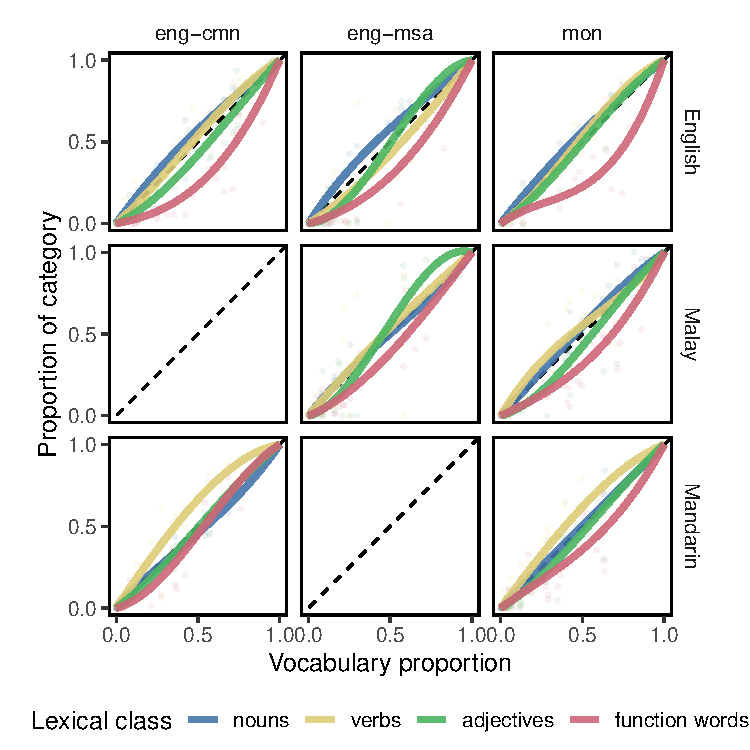
\includegraphics[width=240pt]{figs/my_prop-1} 

}

\caption[Syntactic category composition curves for each language and participant group from the Malaysian sample]{Syntactic category composition curves for each language and participant group from the Malaysian sample. Lines show model fits. The dashed line represents no bias. mon: monolinguals.}\label{fig:my_prop}
\end{figure}
\end{CodeChunk}

To illustrate our analytic approach, syntactic category composition
curves are shown in Figure \ref{fig:my_prop}, reflecting the proportion
of each syntactic category produced by each child as a function of the
proportion of all items produced by the child. As found in previous work
(Frank et al., 2021, ch.~11), children exhibited a negative function
word bias across all languages and groups. Children also showed a
positive noun bias in English and a positive predicate bias in Mandarin,
while the size of the noun and predicate biases was close to zero for
Malay.

\begin{CodeChunk}
\begin{figure}[t]

{\centering 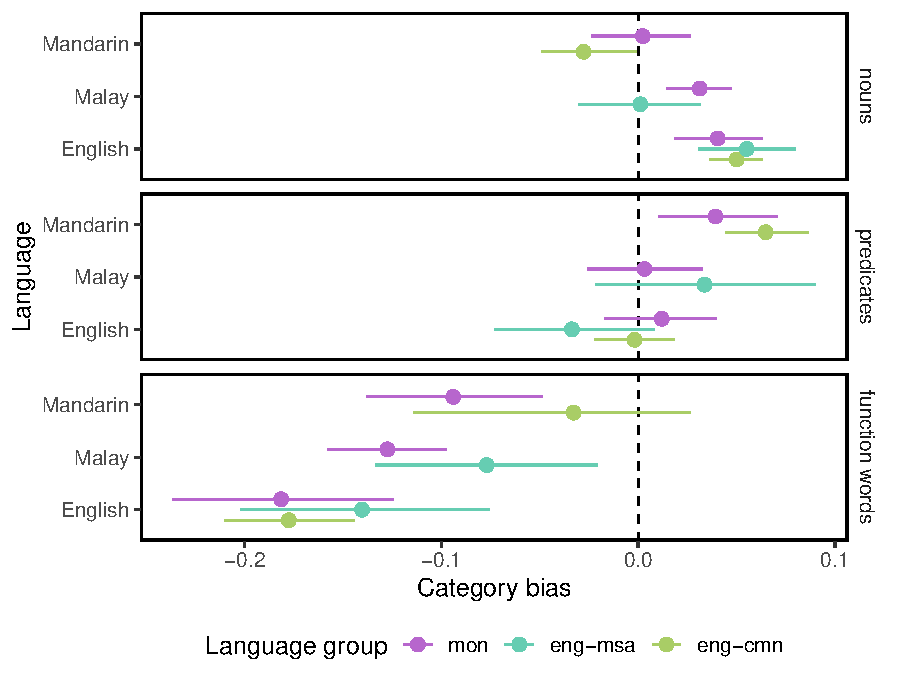
\includegraphics[width=240pt]{figs/my_bias-1} 

}

\caption[Estimated syntactic category biases for each language and participant group from the Malaysian sample]{Estimated syntactic category biases for each language and participant group from the Malaysian sample. Ranges indicate bootstrapped 95\% confidence intervals. The dashed line represents no bias. mon: monolinguals.}\label{fig:my_bias}
\end{figure}
\end{CodeChunk}

To visualise the sizes of the syntactic category biases, Figure
\ref{fig:my_bias} shows model estimates for each language and
participant group. We examined the following comparisons in our
permutation test: bilinguals vs corresponding monolinguals,
Mandarin--English vs Malay--English bilinguals, and English vs
Mandarin/Malay within bilingual groups. Although visually there appears
to be variation across participant groups, there were not in fact any
statistically significant differences across groups for any syntactic
category in any language (all \(p\) ≥ .610). In other words,
participants with different language backgrounds exhibited
similarly-sized category biases for any given language, and bilinguals
did not differ in their category biases between their two languages.
This result corroborates and extends findings from Chai et al. (2021),
who did not find effects in production.\footnote{A similar analysis for
  comprehension data also did not reveal any significant differences
  between groups, even for the between-bilinguals condition found to
  have an effect by Chai et al. (2021).}

The lack of an effect is nonetheless surprising, since Mandarin and
English have been found (in other studies) to have large differences in
category bias sizes. There are a few possible reasons for this null
finding. First, the category bias effect sizes may have been influenced
by language exposure. Although we controlled for the effect of exposure
statistically through matching, it is plausible that greater exposure to
one language may entrain a larger modulation of category bias sizes in
the other language for a bilingual. Because children with different
exposure distributions were collapsed together in this analysis, it was
not possible to determine the contribution of language exposure to
category bias sizes. Second, it is possible that there was not enough
power to find a significant effect due to the small sample size. To
address these issues, we shifted to a larger dataset in our second
analysis, which allowed us to bin participants by language exposure.

\section{Analysis 2: Varying language
exposures}\label{analysis-2-varying-language-exposures}

In this analysis, we examined the effect of language exposure by binning
children by language exposure proportions within a large sample of
English--Spanish bilinguals. If category bias were affected by
cross-linguistic influence, we should see the largest modulation for
children who receive the most exposure to another language. In addition,
across a bilingual child's two languages, we should see the biggest
difference in bias sizes for children with the biggest imbalance in
language exposure.

\subsection{Dataset}\label{dataset-1}

The dataset for this analysis included data from Hoff et al. (2012),
Hoff et al. (2018), and Marchman et al. (2004) on English--Spanish
bilingual children. It includes 1800 children (917 boys) from the US
aged 17--49 months. We binned participants into five bins by language
exposure, and matched participants across bins. This resulted in a final
sample of 1450 children (741 boys).

\subsection{Results and discussion}\label{results-and-discussion-1}

\begin{CodeChunk}
\begin{figure}[t]

{\centering 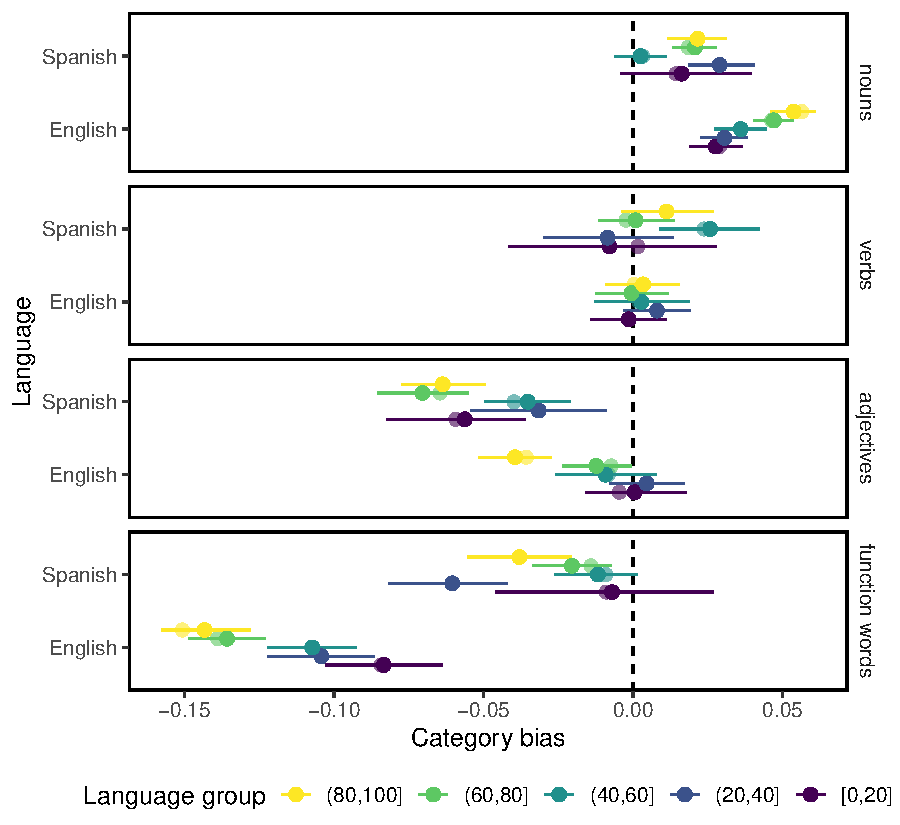
\includegraphics[width=240pt]{figs/us_bias-1} 

}

\caption[Estimated syntactic category biases for each language and English exposure proportion from the US sample]{Estimated syntactic category biases for each language and English exposure proportion from the US sample. Ranges indicate bootstrapped 95\% confidence intervals. The dashed line represents no bias.}\label{fig:us_bias}
\end{figure}
\end{CodeChunk}

Figure \ref{fig:us_bias} shows model estimates for each language and
participant group. We examined the following comparisons in our
permutation test: (80,100{]} vs other exposure bins for each language,
and Spanish vs English for each corresponding exposure bin (i.e.,
{[}0,20{]} for English corresponds to (80,100{]} for Spanish). Four
comparisons survived the correction for multiple comparisons. Children
exposed to (80,100{]} percent English had more negative function word
biases and more positive noun biases than children exposed to {[}0,20{]}
percent English (both \(p\) \textless{} .001). Children exposed to
(80,100{]} percent English also had more positive noun biases than
children exposed to (20,40{]} percent English (\(p\) = .010). Finally,
children exposed to (80,100{]} percent English had more negative
function word biases in English than in Spanish (\(p\) \textless{}
.001). Eight other comparisons were significant prior to correction but
did not survive the correction (all \(p\) within {[}.069, .157{]}).

As hypothesised, we found significant modulation of category biases in
English for children exposed to more Spanish---i.e., the category biases
of children exposed to \textgreater80\% Spanish had \emph{English}
category biases that were more like those of Spanish, in comparison to
children exposed to ≤20\% Spanish. In addition, children with the
biggest imbalance in language exposure (\textgreater80\% English, ≤20\%
Spanish) showed the biggest difference in category biases across their
two languages. Interestingly, these effects were asymmetric---children
exposed to more English did not show any modulation of their category
biases in Spanish, and children exposed to mostly Spanish did not show a
big difference in category biases across their languages. One reason for
this asymmetry may be the statuses of the two languages---in the US,
English is the majority language while Spanish is a minority language.
The difference in language status may drive contextual differences in
which these languages appear---for example, Spanish may be spoken more
at home, while English may be spoken more in community settings. Thus,
the distributional properties of Spanish may not change regardless of
language exposure, while those for English may shift from more
idiolectal at lower exposure levels to more standard at higher exposure
levels. To understand the possible role of context, we turn to varying
the environmental context in our third analysis.

\section{Analysis 3: Varying environmental
contexts}\label{analysis-3-varying-environmental-contexts}

In this analysis, we examine the effect of broad environmental context
by comparing children who are acquiring the same pairs of languages but
who are being raised in different countries. If environmental factors
(e.g., language status) affect category bias, we should observe
differences in bias sizes for children in different countries, even if
they are acquiring the same combination of languages, once factors such
as age and language exposure are controlled for.

\subsection{Dataset}\label{dataset-2}

The dataset for this analysis included data from Siow et al. (2023) on
bilingual children in the UK and Continental Europe. We chose a subset
of language combinations that had data from both the UK and another
European country: English--Dutch (UK/the Netherlands), English--German
(UK/Germany), and English--Spanish (UK/Spain). The data include 554
children (273 boys) aged 4--54 months. As in Analysis 1, we thresholded
language exposure values at 10\% and grouped participants by language
combination and country of origin, performing matching within each
language combination. We also included the small set of UK monolingual
English children for completeness. This resulted in a final sample of
353 children (190 boys).

\subsection{Results and discussion}\label{results-and-discussion-2}

\begin{CodeChunk}
\begin{figure}[t]

{\centering 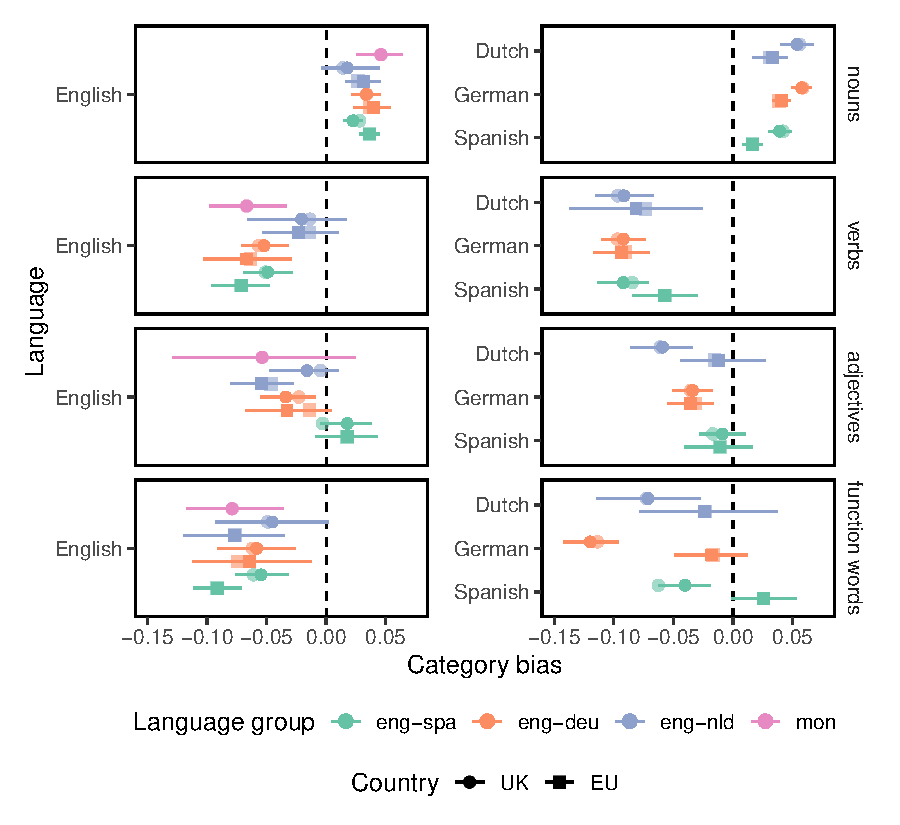
\includegraphics[width=240pt]{figs/ox_bias-1} 

}

\caption[Estimated syntactic category biases for each language and exposure proportion from the European sample]{Estimated syntactic category biases for each language and exposure proportion from the European sample. Ranges indicate bootstrapped 95\% confidence intervals. The dashed line represents no bias. mon: monolinguals.}\label{fig:ox_bias}
\end{figure}
\end{CodeChunk}

Figure \ref{fig:ox_bias} shows model estimates for each language and
participant group. We examined comparisons between children from
different countries within each language combination. For completeness,
we also compared English category biases for all groups against the UK
monolingual English group, although the imbalance in group size and
other covariates means that these comparisons may be less reliable. Only
one comparison survived the correction for multiple comparisons:
function words in German for children from the UK vs Germany (\(p\)
\textless{} .001). Two other comparisons were significant prior to
correction but did not survive the correction: function words in Spanish
for children from the UK vs Spain (\(p\) = .072), and nouns in German
for children from the UK vs Germany (\(p\) = .310).

As hypothesised, we found an effect of environmental context, such that
children acquiring English and German exhibited different function word
biases depending on whether they were growing up in the UK or in
Germany. The lack of an effect for any other comparison may again be due
to a lack of power, as is evidenced by the somewhat large confidence
intervals. A larger sample may be able to provide narrower confidence
intervals, and uncover smaller effects that the current sample cannot.
It may also be the case that the effect depends on the specific language
combination, such that there is an interaction between the linguistic
and contextual factors on category bias variation.

\section{General discussion}\label{general-discussion}

Across our three analyses, we found evidence that syntactic category
biases could vary across a bilingual's two languages, and that these
biases could be modulated cross-linguistically (Analysis 2), supporting
H1c---category biases are affected by intra- and inter-language factors.
We also found that category biases were sometimes influenced by
children's environmental context (Analysis 3), supporting H2b---category
biases are affected by contextual factors. Taken together, the supported
hypotheses suggest that linguistic and contextual factors both play a
role in shaping the syntactic composition of children's early
vocabularies. This finding also provides an imperative for language
acquisition researchers to be more thorough and precise with their
description of the language learning environment of their study
populations, since background variables other than language may affect
their language outcomes (see Titone \& Tiv, 2023).

Our results also suggested that factors affecting category biases were
not uniform across language combinations (Analyses 1 and 3). This
observation is perhaps unsurprising---since some language pairs have
very similar category bias sizes even for monolinguals, any
cross-linguistic influence would not be apparent, whereas other language
pairs have very divergent bias sizes, permitting the observation of
cross-linguistic influence. This result also emphasises the importance
of surveying a broader set of language combinations in bilingualism
research, since some true effects may not be elicitable in particular
language pairs. A majority of bilingualism research has focused on
bilinguals acquiring English and another language (including the present
work!), which does not comprehensively cover the possible relationships
between a bilingual's two languages; a much broader scope of
investigation would be necessary to understand the generalisability of
various effects related to bilingualism.

Methodologically, the analytic method employed in the present work
provided a means to directly investigate the over- or
under-representation of syntactic categories in children's early
vocabularies. This method allowed for a measurement that has a closer
link with the construct of interest---that is, whether particular
syntactic categories are privileged in children's word learning
processes---since the number of potentially learnable words is
controlled for. However, this approach also required the use of
non-parametric statistics, since the bias sizes must be estimated from
whole samples (rather than individual children); this requirement in
turn meant that we had to control for covariates via matching (instead
of direct modelling). As matching is typically constrained by the
subgroup with the smallest size, our approach may have limited the power
of our analyses, as indeed was suggested by the large confidence
intervals obtained. Future work should involve larger sample sizes in
order to improve the ability of such analyses to detect true effects,
although we acknowledge that the task of collecting data from young
bilinguals is often difficult as population sizes tend to be smaller
than other potential populations of interest.

Nonetheless, the current set of analyses represent an attempt at
disentangling a number of potential factors contributing to differential
learning of words from different syntactic categories in young children,
providing evidence that linguistic and contextual factors are both
important to consider in language acquisition. These results also show
the importance of studying bilingual populations to understand learning
processes theorised to underlie language acquisition in all contexts,
since any such theory must be able to account for the simultaneous
acquisition of multiple languages; the significance of this statement is
underscored by the fact that language acquisition research on
monolinguals is much more common than that on multilinguals, even though
many more children grow up in multilingual rather than monolingual
settings (Kidd \& Garcia, 2022). In fact, studying bilinguals may afford
approaches that are not possible with monolinguals, as evidenced by the
present work. We anticipate that an increasing emphasis on understudied
language settings, combined with increasing statistical sophistication
and increasing open science practices, will serve to improve the
generalisability, accuracy, and rigour of our theories of language
acquisition.

\newpage

\section{Acknowledgements}\label{acknowledgements}

We would like to thank the data contributors as well as developers and
maintainers of Wordbank, whose efforts towards open science have made
this research possible.

\section{References}\label{references}

\setlength{\parindent}{-0.1in} 
\setlength{\leftskip}{0.125in}

\noindent

\phantomsection\label{refs}
\begin{CSLReferences}{1}{0}
\bibitem[\citeproctext]{ref-barnesVocabularyGrowthComposition2013}
Barnes, J., \& Garcia, I. (2013). Vocabulary growth and composition in
monolingual and bilingual {Basque} infants and toddlers.
\emph{International Journal of Bilingualism}, \emph{17}(3), 357--374.
\url{https://doi.org/10.1177/1367006912438992}

\bibitem[\citeproctext]{ref-batesDevelopmentalStylisticVariation1994}
Bates, E., Marchman, V., Thal, D., Fenson, L., Dale, P., Reznick, J. S.,
Reilly, J., \& Hartung, J. (1994). Developmental and stylistic variation
in the composition of early vocabulary. \emph{Journal of Child
Language}, \emph{21}(1), 85--123.
\url{https://doi.org/10.1017/s0305000900008680}

\bibitem[\citeproctext]{ref-benjaminiControllingFalseDiscovery1995}
Benjamini, Y., \& Hochberg, Y. (1995). Controlling the {False Discovery
Rate}: {A Practical} and {Powerful Approach} to {Multiple Testing}.
\emph{Journal of the Royal Statistical Society: Series B
(Methodological)}, \emph{57}(1), 289--300.
\url{https://doi.org/10.1111/j.2517-6161.1995.tb02031.x}

\bibitem[\citeproctext]{ref-bornsteinCrossLinguisticAnalysisVocabulary2004}
Bornstein, M. H., Cote, L. R., Maital, S., Painter, K., Park, S.-Y.,
Pascual, L., Pêcheux, M.-G., Ruel, J., Venuti, P., \& Vyt, A. (2004).
Cross-{Linguistic Analysis} of {Vocabulary} in {Young Children}:
{Spanish}, {Dutch}, {French}, {Hebrew}, {Italian}, {Korean}, and
{American English}. \emph{Child Development}, \emph{75}(4), 1115--1139.
\url{https://doi.org/10.1111/j.1467-8624.2004.00729.x}

\bibitem[\citeproctext]{ref-caselliCrosslinguisticStudyEarly1995}
Caselli, M. C., Bates, E., Casadio, P., Fenson, J., Fenson, L., Sanderl,
L., \& Weir, J. (1995). A cross-linguistic study of early lexical
development. \emph{Cognitive Development}, \emph{10}(2), 159--199.
\url{https://doi.org/10.1016/0885-2014(95)90008-X}

\bibitem[\citeproctext]{ref-casillasLittleEvidenceNoun2024}
Casillas, M., Foushee, R., Méndez Girón, J., Polian, G., \& Brown, P.
(2024). Little evidence for a noun bias in {Tseltal} spontaneous speech.
\emph{First Language}, \emph{44}(6), 600--628.
\url{https://doi.org/10.1177/01427237231216571}

\bibitem[\citeproctext]{ref-chaiExtralinguisticModulationEnglish2021}
Chai, J. H., Low, H. M., Wong, T. P., Onnis, L., \& Mayor, J. (2021).
Extra-linguistic modulation of the {English} noun-bias: Evidence from
{Malaysian} bilingual infants and toddlers. \emph{Journal of Cultural
Cognitive Science}, \emph{5}(1), 49--64.
\url{https://doi.org/10.1007/s41809-021-00078-5}

\bibitem[\citeproctext]{ref-chanPredictingTwoMandarinEnglish2010}
Chan, W. H., \& Nicoladis, E. (2010). Predicting two {Mandarin-English}
bilingual children's first 50 words: {Effects} of frequency and relative
exposure in the input. \emph{International Journal of Bilingualism},
\emph{14}(2), 237--270. \url{https://doi.org/10.1177/1367006910363059}

\bibitem[\citeproctext]{ref-choiEarlyAcquisitionVerbs1995}
Choi, S., \& Gopnik, A. (1995). Early acquisition of verbs in {Korean}:
A cross-linguistic study. \emph{Journal of Child Language},
\emph{22}(3), 497--529. \url{https://doi.org/10.1017/S0305000900009934}

\bibitem[\citeproctext]{ref-fensonMacArthurBatesCommunicativeDevelopment2007}
Fenson, L., Marchman, V. A., Thal, D. J., Dale, P. S., Reznick, J. S.,
\& Bates, E. (2007). \emph{{MacArthur-Bates Communicative Development
Inventories}: {User}'s {Guide} and {Technical Manual}}. Paul H. Brookes
Publishing Company.

\bibitem[\citeproctext]{ref-fortinAppliedComparisonLargescale2021}
Fortin, S. P., Johnston, S. S., \& Schuemie, M. J. (2021). Applied
comparison of large-scale propensity score matching and cardinality
matching for causal inference in observational research. \emph{BMC
Medical Research Methodology}, \emph{21}(1), 109.
\url{https://doi.org/10.1186/s12874-021-01282-1}

\bibitem[\citeproctext]{ref-frankWordbankOpenRepository2017}
Frank, M. C., Braginsky, M., Yurovsky, D., \& Marchman, V. A. (2017).
Wordbank: An open repository for developmental vocabulary data.
\emph{Journal of Child Language}, \emph{44}(3), 677--694.
\url{https://doi.org/10.1017/S0305000916000209}

\bibitem[\citeproctext]{ref-frankVariabilityConsistencyEarly2021}
Frank, M. C., Braginsky, M., Yurovsky, D., \& Marchman, V. A. (2021).
\emph{Variability and {Consistency} in {Early Language Learning}: {The
Wordbank Project}}. MIT Press.

\bibitem[\citeproctext]{ref-gentnerWhyNounsAre1982}
Gentner, D. (1982). Why nouns are learned before verbs: {Linguistic}
relativity versus natural partitioning. \emph{Language}, \emph{2},
301--334.

\bibitem[\citeproctext]{ref-goldfieldNounBiasMaternal1993}
Goldfield, B. A. (1993). Noun bias in maternal speech to one-year-olds.
\emph{Journal of Child Language}, \emph{20}(1), 85--99.
\url{https://doi.org/10.1017/S0305000900009132}

\bibitem[\citeproctext]{ref-hoffDualLanguageExposure2012}
Hoff, E., Core, C., Place, S., Rumiche, R., Señor, M., \& Parra, M.
(2012). Dual language exposure and early bilingual development.
\emph{Journal of Child Language}, \emph{39}(1), 1--27.
\url{https://doi.org/10.1017/S0305000910000759}

\bibitem[\citeproctext]{ref-hoffWhatExplainsCorrelation2018}
Hoff, E., Quinn, J. M., \& Giguere, D. (2018). What {Explains} the
{Correlation Between Growth} in {Vocabulary} and {Grammar}? {New
Evidence From Latent Change Score Analyses} of {Simultaneous Bilingual
Development}. \emph{Developmental Science}, \emph{21}(2).
\url{https://doi.org/10.1111/desc.12536}

\bibitem[\citeproctext]{ref-kiddHowDiverseChild2022}
Kidd, E., \& Garcia, R. (2022). How diverse is child language
acquisition research? \emph{First Language}, \emph{42}(6), 703--735.
\url{https://doi.org/10.1177/01427237211066405}

\bibitem[\citeproctext]{ref-kimEarlyLexicalDevelopment2000}
Kim, M., McGREGOR, K. K., \& Thompson, C. K. (2000). Early lexical
development in {English-} and {Korean-speaking} children:
Language-general and language-specific patterns. \emph{Journal of Child
Language}, \emph{27}(2), 225--254.
\url{https://doi.org/10.1017/S0305000900004104}

\bibitem[\citeproctext]{ref-klammlerSizeCompositionProductive2011}
Klammler, A., \& Schneider, S. (2011). The size and composition of the
productive holophrastic lexicon: {German}--{Italian} bilingual
acquisition vs. {Italian} monolingual acquisition. \emph{International
Journal of Bilingual Education and Bilingualism}, \emph{14}(1), 69--88.
\url{https://doi.org/10.1080/13670051003692840}

\bibitem[\citeproctext]{ref-lavinEastWestRole2006}
Lavin, T. A., Hall, D. G., \& Waxman, S. R. (2006). East and {West}: {A
Role} for {Culture} in the {Acquisition} of {Nouns} and {Verbs}. In K.
A. Hirsh-Pasek \& R. M. Golinkoff (Eds.), \emph{Action {Meets Word}:
{How} children learn verbs} (p. 0). Oxford University Press.
\url{https://doi.org/10.1093/acprof:oso/9780195170009.003.0021}

\bibitem[\citeproctext]{ref-leveyFirstWordsProduced2003}
Levey, S., \& Cruz, D. (2003). The {First Words Produced} by {Children}
in {Bilingual English}/{Mandarin Chinese Environments}.
\emph{Communication Disorders Quarterly}, \emph{24}(3), 129--136.
\url{https://doi.org/10.1177/15257401030240030401}

\bibitem[\citeproctext]{ref-lucasExploringNounBias2008}
Lucas, R. I. G., \& Bernardo, A. B. I. (2008). Exploring {Noun Bias} in
{Filipino}---{English Bilingual Children}. \emph{The Journal of Genetic
Psychology}, \emph{169}(2), 149--164.
\url{https://doi.org/10.3200/GNTP.169.2.149-164}

\bibitem[\citeproctext]{ref-marchmanMacArthurBatesCommunicativeDevelopment2023}
Marchman, V. A., Dale, P., \& Fenson, L. (2023). \emph{{MacArthur-Bates
Communicative Development Inventories User}'s {Guide} and {Technical
Manual}} (3rd edition). Brookes Publishing Co.

\bibitem[\citeproctext]{ref-marchmanLanguagespecificNatureGrammatical2004}
Marchman, V. A., Martinez-Sussmann, C., \& Dale, P. S. (2004). The
language-specific nature of grammatical development: Evidence from
bilingual language learners. \emph{Developmental Science}, \emph{7}(2),
212--224. \url{https://doi.org/10.1111/j.1467-7687.2004.00340.x}

\bibitem[\citeproctext]{ref-mayorStatisticalEstimateInfant2011}
Mayor, J., \& Plunkett, K. (2011). A statistical estimate of infant and
toddler vocabulary size from {CDI} analysis. \emph{Developmental
Science}, \emph{14}(4), 769--785.
\url{https://doi.org/10.1111/j.1467-7687.2010.01024.x}

\bibitem[\citeproctext]{ref-nicoladisEvidenceBilingualChild2001}
Nicoladis, E. (2001). Evidence from a bilingual child: {Finding} first
words in the input. In J. Cenoz \& F. Genesee (Eds.), \emph{Trends in
{Bilingual Acquisition}} (pp. 131--147). John Benjamins Publishing
Company. \url{https://doi.org/10.1075/tilar.1.08nic}

\bibitem[\citeproctext]{ref-ozcanEarlyLexicalComposition2016}
Özcan, F. H., Altinkamiş, F., \& Gillis, S. (2016). Early lexical
composition of {Turkish-Dutch} bilinguals: {Nouns} before verbs or verbs
before nouns. \emph{Poznan Studies in Contemporary Linguistics},
\emph{52}(4), 583--604. \url{https://doi.org/10.1515/psicl-2016-0023}

\bibitem[\citeproctext]{ref-rassenSimultaneouslyAssessingIntended2011}
Rassen, J. A., Solomon, D. H., Glynn, R. J., \& Schneeweiss, S. (2011).
Simultaneously assessing intended and unintended treatment effects of
multiple treatment options: A pragmatic {``matrix design.''}
\emph{Pharmacoepidemiology and Drug Safety}, \emph{20}(7), 675--683.
\url{https://doi.org/10.1002/pds.2121}

\bibitem[\citeproctext]{ref-setohContrastingLexicalBiases2021}
Setoh, P., Cheng, M., Bornstein, M. H., \& Esposito, G. (2021).
Contrasting lexical biases in bilingual {English}--{Mandarin} speech:
{Verb-biased} mothers, but noun-biased toddlers. \emph{Journal of Child
Language}, \emph{48}(6), 1185--1208.
\url{https://doi.org/10.1017/S0305000920000720}

\bibitem[\citeproctext]{ref-siowDoubleItVocabulary2023}
Siow, S., Gillen, N. A., Lepădatu, I., \& Plunkett, K. (2023). Double it
up: {Vocabulary} size comparisons between {UK} bilingual and monolingual
toddlers. \emph{Infancy}, \emph{28}(6), 1030--1051.
\url{https://doi.org/10.1111/infa.12562}

\bibitem[\citeproctext]{ref-tanRoleTranslationEquivalents2024}
Tan, A. W. M., Marchman, V. A., \& Frank, M. C. (2024). The role of
translation equivalents in bilingual word learning. \emph{Developmental
Science}, \emph{27}(4), e13476. \url{https://doi.org/10.1111/desc.13476}

\bibitem[\citeproctext]{ref-tardifNounsAreNot1996}
Tardif, T. (1996). Nouns {Are Not Always Learned Before Verbs}:
{Evidence From Mandarin Speakers}' {Early Vocabularies}.
\emph{Developmental Psychology}, \emph{32}(3), 492--504.
\url{https://doi.org/10.1037/0012-1649.32.3.492}

\bibitem[\citeproctext]{ref-tardifPuttingNounBias1999}
Tardif, T., Gelman, S. A., \& Xu, F. (1999). Putting the "{Noun Bias}"
in {Context}: {A Comparison} of {English} and {Mandarin}. \emph{Child
Development}, \emph{70}(3), 620--635.
\url{https://www.jstor.org/stable/1132149}

\bibitem[\citeproctext]{ref-tardifCaregiverSpeechChildrens1997}
Tardif, T., Shatz, M., \& Naigles, L. (1997). Caregiver speech and
children's use of nouns versus verbs: {A} comparison of {English},
{Italian}, and {Mandarin}. \emph{Journal of Child Language},
\emph{24}(3), 535--565. \url{https://doi.org/10.1017/S030500099700319X}

\bibitem[\citeproctext]{ref-titoneRethinkingMultilingualExperience2023}
Titone, D. A., \& Tiv, M. (2023). Rethinking multilingual experience
through a {Systems Framework} of {Bilingualism}. \emph{Bilingualism:
Language and Cognition}, \emph{26}(1), 1--16.
\url{https://doi.org/10.1017/S1366728921001127}

\bibitem[\citeproctext]{ref-tsuiAreTranslationEquivalents2022}
Tsui, R. K.-Y., Gonzalez-Barrero, A. M., Schott, E., \& Byers-Heinlein,
K. (2022). Are translation equivalents special? {Evidence} from
simulations and empirical data from bilingual infants. \emph{Cognition},
\emph{225}, 105084.
\url{https://doi.org/10.1016/j.cognition.2022.105084}

\bibitem[\citeproctext]{ref-waxmanAreNounsLearned2013}
Waxman, S. R., Fu, X., Arunachalam, S., Leddon, E., Geraghty, K., \&
Song, H. (2013). Are {Nouns Learned Before Verbs}? {Infants Provide
Insight} into a {Longstanding Debate}. \emph{Child Development
Perspectives}, \emph{7}(3), 10.1111/cdep.12032.
\url{https://doi.org/10.1111/cdep.12032}

\bibitem[\citeproctext]{ref-waxmanHowEarlyInfants2016}
Waxman, S. R., Fu, X., Ferguson, B., Geraghty, K., Leddon, E., Liang,
J., \& Zhao, M.-F. (2016). How {Early} is {Infants}' {Attention} to
{Objects} and {Actions Shaped} by {Culture}? {New Evidence} from
24-{Month-Olds Raised} in the {US} and {China}. \emph{Frontiers in
Psychology}, \emph{7}. \url{https://doi.org/10.3389/fpsyg.2016.00097}

\bibitem[\citeproctext]{ref-xinNounVerbBias2010}
Xin, J., \& Lucas, R. I. G. (2010). Noun versus {Verb Bias} in
{Mandarin- English Bilingual Pre-School Children}. \emph{TESOL Journal},
\emph{3}.

\bibitem[\citeproctext]{ref-xuanLanguagespecificNounBias2013}
Xuan, L., \& Dollaghan, C. (2013). Language-specific noun bias: Evidence
from bilingual children. \emph{Journal of Child Language}, \emph{40}(5),
1057--1075. \url{https://doi.org/10.1017/S0305000912000529}

\end{CSLReferences}

\bibliographystyle{apacite}


\end{document}
